\documentclass[14pt, a4paper]{extarticle}
\usepackage{GOST}
\usepackage{array}
\usepackage{verbatim}
\usepackage[detect-all]{siunitx}
\usepackage{amsmath}
\usepackage{amssymb}
\usepackage[utf8]{inputenc}
\usepackage{hyperref}
\usepackage{tempora}

\makeatletter
\renewcommand\@biblabel[1]{#1.}
\makeatother

\usepackage{listings}
\lstset{ 
	language=c,
	basicstyle=\small\sffamily, 
	numbers=left, 
	numberstyle=\tiny,
	stepnumber=1,
	numbersep=5pt,
	showspaces=false,            
	showstringspaces=false,      
	showtabs=false,             
	frame=single,            % рисовать рамку вокруг кода
	tabsize=4,      
	commentstyle=\color{green},
	keywordstyle=\color{blue}\textbf,
	numberstyle=\scriptsize\color{gray}, % the style that is used for the line-numbers
	rulecolor=\color{black},
	captionpos=t,
	breaklines=true,         % автоматически переносить строки 
	breakatwhitespace=false, % переносить строки по пробелу
	escapeinside={\#*}{*)} 
}

\begin{document}
	
\begin{table}[ht]
	\centering
	\begin{tabular}{|c|p{400pt}|} 
		\hline
		\begin{tabular}[c]{@{}c@{}} 
\includegraphics[scale=1]{baum.jpg} \\\end{tabular} &
		\footnotesize\begin{tabular}[c]{@{}c@{}}\textbf{Министерство~науки~и~высшего~образования~Российской~Федерации}\\\textbf{Федеральное~государственное~бюджетное~образовательное~учреждение}\\\textbf{~высшего~образования}\\\textbf{«Московский~государственный~технический~университет}\\\textbf{имени~Н.Э.~Баумана}\\\textbf{(национальный~исследовательский~университет)»}\\\textbf{(МГТУ~им.~Н.Э.~Баумана)}\\\end{tabular}  \\
		\hline
	\end{tabular}
\end{table}
\noindent\rule{\textwidth}{4pt}
\noindent\rule[14pt]{\textwidth}{1pt}
\hfill 
\noindent
\makebox{ФАКУЛЬТЕТ~}%
\makebox[\textwidth][l]{\underline{~«Информатика и системы управления»~~~~~~~~~~~~~~~~~~~~~~~~~~~~~~~~~}}%
\\
\noindent
\makebox{КАФЕДРА~}%
\makebox[\textwidth][l]{\underline{~«Операционные системы»~}}%


\begin{center}
	\vspace{1.5cm}
	{\bf\huge Отчёт\par}
	{\bf\Large по лабораторной работе № 5\par}
	\vspace{0.7cm}
\end{center}

\noindent
\makebox{\large{\bf Название:}~~~}
\makebox[\textwidth][l]{\large\underline{~ Буферизованный и не буферизованный ввод-вывод~}}\\


\noindent
\makebox{\large{\bf Дисциплина:}~~~}
\makebox[\textwidth][l]{\large\underline{~Операционные системы~}}\\

\vspace{1.5cm}
\noindent
\begin{tabular}{l c c c c c}
	Студент      & ~ИУ7-65Б~               & \hspace{2.5cm} & \hspace{2cm}                 & &  Д.В. Сусликов \\\cline{2-2}\cline{4-4} \cline{6-6} 
	\hspace{3cm} & {\footnotesize(Группа)} &                & {\footnotesize(Подпись, дата)} & & {\footnotesize(И.О. Фамилия)}
\end{tabular}

\noindent
\begin{tabular}{l c c c c}
	Преподователь & \hspace{5cm}   & \hspace{2cm}                 & & ~~~Н.Ю. Рязанова~~~\\\cline{3-3} \cline{5-5} 
	\hspace{3cm}  &                & {\footnotesize(Подпись, дата)} & & {\footnotesize(И.О. Фамилия)}
\end{tabular}

\vspace{0.6cm}
\begin{center}	
	\vfill
	\large \textit {Москва, 2021}
\end{center}

\thispagestyle {empty}
\pagebreak

% ВВЕДЕНИЕ
\clearpage
\textbf{Программа 1} \par

\textbf{Листинг:}
\begin{lstlisting}
	#include <stdio.h>
	#include <fcntl.h>
	
	int main()
	{
		int fd = open("alph.txt", O_RDONLY);
		
		FILE *fs1 = fdopen(fd, "r");
		char buff1[20];
		setvbuf(fs1, buff1, _IOFBF, 20);
		
		FILE *fs2 = fdopen(fd, "r");
		char buff2[20];
		setvbuf(fs2, buff2, _IOFBF, 20);
		
		int flag1 = 1, flag2 = 2;
		while(flag1 == 1 || flag2 == 1)
		{
			char c;
			flag1 = fscanf(fs1, "%c", &c);
			if (flag1 == 1)
			fprintf(stdout, "%c", c);
			
			flag2 = fscanf(fs2, "%c", &c);
			if (flag2 == 1) 
			fprintf(stdout, "%c", c); 
		}
		
		return 0;
	}
\end{lstlisting}\newpage

\begin{figure}[h!]
	\center{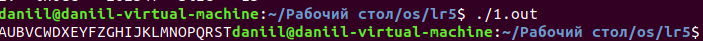
\includegraphics[scale=0.6]{examples/1.png}}
	\caption{Результат  программы 1}
\end{figure}\par

Системный вызов open() создает дескриптор открытого на чтение файла. Open() возвращает индекс в массиве fd структуры files\_struct. fdopen() создает структуры типа FILE(fs1 и fs2), которые ссылаются на дескриптор, созданный системным вызовом open.

Создаём буферы buff1 и buff2 размером 20 байт. С помощью setbuv задаём соответствующие буферы для дескрипторов fs1 и fs2 и устанавливаем тип буферизации \_IOFBF (полная буферизация).

Далее в цикле fscanf() поочерёдно для fs1 и fs2. Так как установлена полная буферизация, то при первом вызове fscanf() буфер будет заполнен полностью, либо вплоть до конца файла, а f\_pos установится на следующий за последним записанным в буфер символ.

При первом вызове fscanf(fs1,"\%c",\&c) в буфер buff1 считаются первые 20 символов (abcdefghijklmnopqrst), запись производится через переменную с, а затем выводится с помощью fprintf, символ 'a'.

При первом вызове fscanf(fs2,"\%c",\&c), в буфер buff2 считываются оставшиеся в файле символы – uvwxyz (в с записывается символ 'u').

Внутри цикла будут поочередно выводится символы издвух буферов до тех пор, пока символы в одном из буферов не закончатся. Тогда на экран будут последовательно выведены оставшиеся символы из другого буфера.

\begin{figure}[h!]
	\center{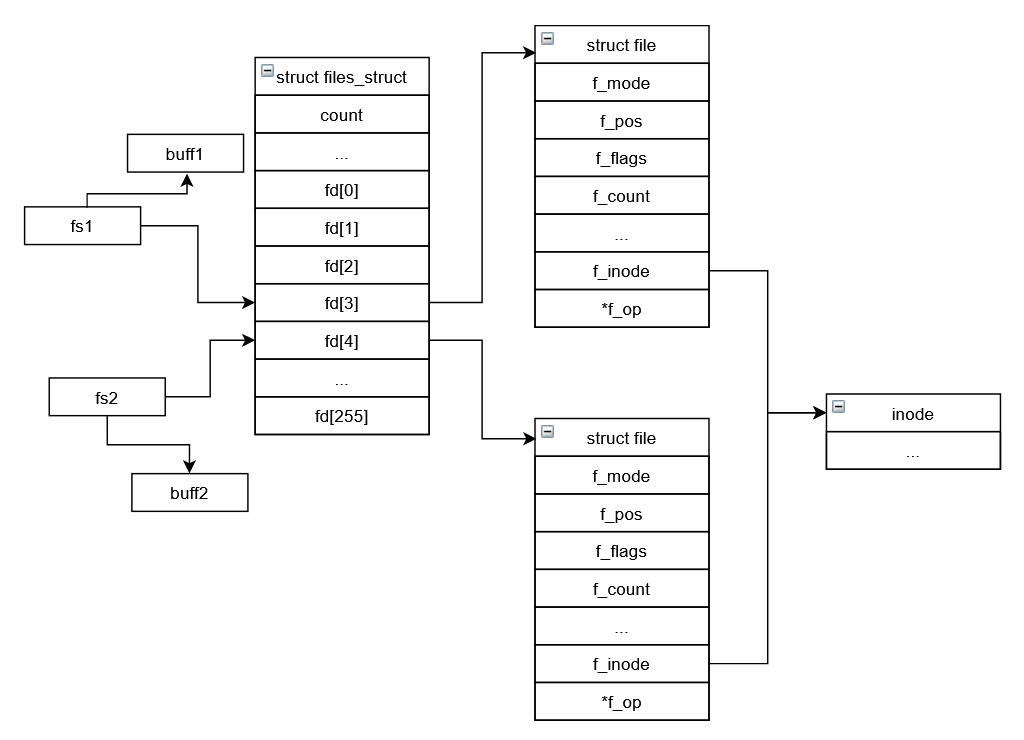
\includegraphics[scale=0.45]{schemes/1.jpg}}
	\caption{Схема связей структур}
\end{figure}\par

\clearpage
\textbf{Листинг:}
\begin{lstlisting}
#include<fcntl.h>

int main()
{
	char c;    
	int fd1 = open("alph.txt", O_RDONLY);
	int fd2 = open("alph.txt", O_RDONLY);
	
	while(read(fd1, &c, 1) == 1 &&read(fd2, &c, 1) == 1)
	{
		write(1, &c, 1);
		write(1, &c, 1);
	}
	return 0;
}
\end{lstlisting}\par

\begin{figure}[h!]
	\center{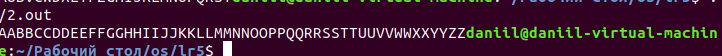
\includegraphics[scale=0.6]{examples/2.png}}
	\caption{Результат программы 2}
\end{figure}\par

Open() создаст два дескриптора одного файла, доступного
только для чтения. Будут созданы две структуры struct file в общесистемной таблице открытых файлов. Таким образом, поля f\_pos в каждой из структур независимы.

В цикле выполнятся read(), считывающий символ и write(), записывающий
символ в стандартный поток. Указатель f\_pos изменяется независимо от другого дескриптора, поэтому каждый символ будет выведен дважды.

\begin{figure}[h!]
	\center{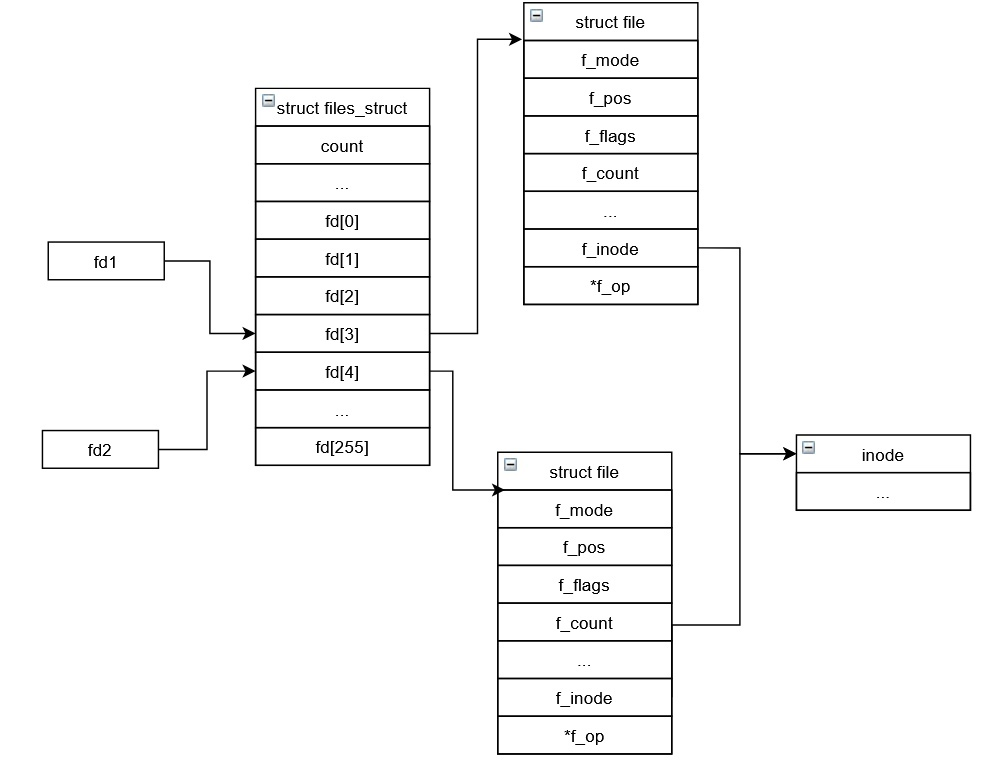
\includegraphics[scale=0.45]{schemes/2.jpg}}
	\caption{Схема связей структур}
\end{figure}\par

\clearpage
\textbf{Листинг:}
\begin{lstlisting}
#include <stdio.h>
#include <stdlib.h>
#include <pthread.h>
#include <fcntl.h>
void *reading(int *fd)
{
	char c;
	while (read(*fd, &c, 1) == 1)
	write(1, &c, 1);
}
int main()
{
	int fd1 = open("alph.txt", O_RDONLY);
	int fd2 = open("alph.txt", O_RDONLY);
	pthread_t thread1;
	
	int stat1 = pthread_create(&thread1, NULL, reading, &fd1);
	if (stat1 != 0)
	{
		printf("Error. Can`t create thread 1\n");
		return -1;
	}
	
	reading(&fd2);
	
	pthread_join(thread1, NULL);
	
	return 0;
}
\end{lstlisting}

\begin{figure}[h!]
	\center{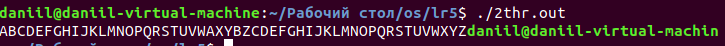
\includegraphics[scale=0.6]{examples/2.2.png}}
	\caption{Результат программы 2 с потоками}
\end{figure}\par
Аналогично программе без потока, вызов open() создаст два независимых
дескриптора открытых файлов, содержащих собственные значения f\_pos. В
результате каждый поток выполнит чтение и запись независимо, что приведет к
повтору каждого символа в результирующей строке.

\newpage
\textbf{Листинг:}
\begin{lstlisting}
	#include <stdio.h>
	#include <sys/stat.h>
	
	int main()
	{
		struct stat stats;
		
		FILE *fp1 = fopen("alphChange.txt", "w");
		stat("alphChange.txt", &stats);
		printf("1:  inode - %d  size - %d\n", (int) stats.st_ino, (int) stats.st_size);
		
		FILE *fp2 = fopen("alphChange.txt", "w");
		stat("alphChange.txt", &stats);
		printf("2:  inode - %d  size - %d\n", (int) stats.st_ino, (int) stats.st_size);
		
		for (char c = 'a'; c <= 'z'; c++) 
		{
			if (c % 2 == 0)
				fprintf(fp1, "%c", c);		
			else
				fprintf(fp2, "%c", c);
		}	
		fclose(fp1);
		stat("alphChange.txt", &stats);
		printf("1:  inode - %d  size - %d\n", (int) stats.st_ino, (int) stats.st_size);
		
		fclose(fp2);
		stat("alphChange.txt", &stats);
		printf("2:  inode - %d  size - %d\n", (int) stats.st_ino, (int) stats.st_size);
		
\end{lstlisting}

\begin{figure}[h!]
	\center{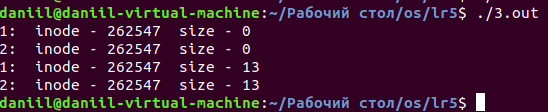
\includegraphics[scale=0.6]{examples/3.png}}
	\caption{Результат программы 3}
\end{figure}\par

Функция fopen() возвращает указатель на
открытый файл. Режим ‘w’ указывает на открытие файла только для записи; 
система помещает указатель в начало файла.
Если файл не существует - пробует его создать. Создаются дескриптора открытых файлов, следовательно, два независимых f\_pos.

Функция fprintf() – функция буферизованного ввода/вывода.
В цикле происходит запись каждого четного символа в один буфер, и нечетного в другой. Запись в файл из буфера
происходит при вызове функции fclose().
Поскольку сначала вызывается fclose(fp1), то буфер, ассоциированный с fp1
будет записан в файл. 

При следующем вызове fclose(fp2) содержимое файла будет
перезаписано, в результате чего в нем окажутся лишь символы из буфера,
связанного с fp2. Таким образом, данные из первого буфера будут утеряны.

\begin{figure}[h!]
	\center{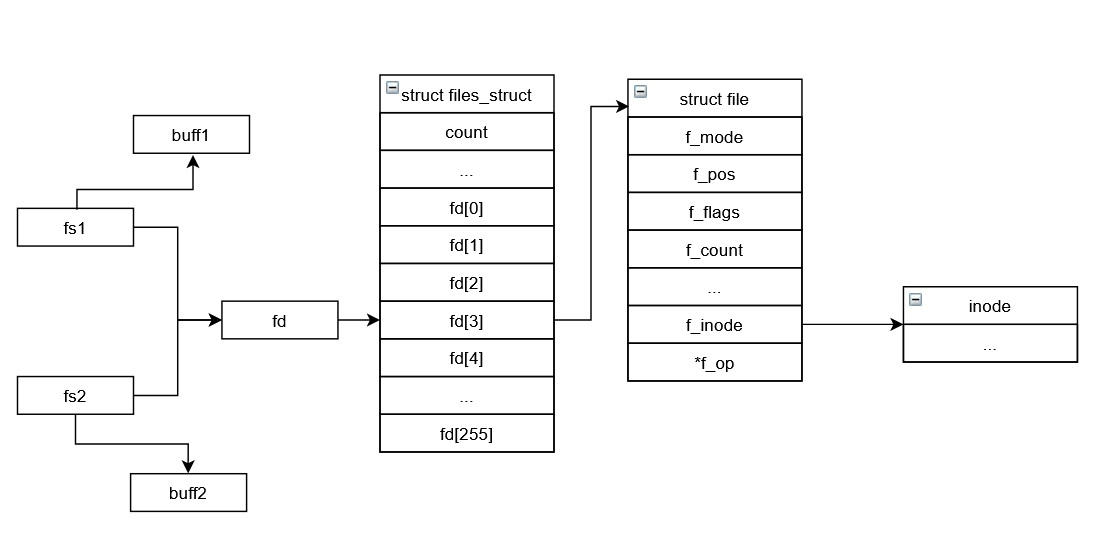
\includegraphics[scale=0.45]{schemes/3.jpg}}
	\caption{Схема связей структур}
\end{figure}\par

\newpage
\textbf{Листинг:}
\begin{lstlisting}
#include <stdio.h>
#include <stdlib.h>
#include <sys/stat.h>
#include <pthread.h>

void *writing(int *fd)
{
	struct stat sb;
	
	FILE *fp = fopen("alphChange.txt", "w");
	stat("alphChange.txt", &sb);
	printf("%d:  inode - %d  size - %d\n", *fd, (int) sb.st_ino, (int)sb.st_size);
	for (char c = 'a'; c <= 'z'; c++)
	{
		if (c % 2 == 0 && *fd % 2 == 1)
		fprintf(fp, "%c", c);
		
		if (c % 2 == 1 && *fd % 2 == 0)
		fprintf(fp, "%c", c);
		
	}
	fclose(fp);
	stat("alphChange.txt", &sb);
	printf("%d:  inode - %d  size - %d\n", *fd, (int) sb.st_ino, (int)sb.st_size);
}

int main()
{
	pthread_t thread1, thread2;
	int fd1 = 1, fd2 = 2;
	
	int stat1 = pthread_create(&thread1, NULL, writing, &fd1);
	if (stat1 != 0)
	{
		printf("Error. Can`t create thread 1\n");
		return -1;
	}
	writing(&fd2);
	
	pthread_join(thread1, NULL);
	
	return 0;
}
	\end{lstlisting}

\begin{figure}[h!]
	\center{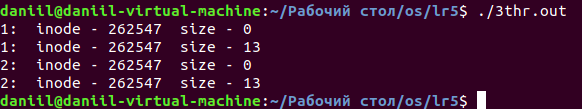
\includegraphics[scale=0.6]{examples/3.2.png}}
	\caption{Результат программы 3 с потоками}
\end{figure}\par

Аналогично программе без потоков, будут созданы два независимых
дескриптора. Каждый из потоков будет выполнять запись символов в
соответствующий буфер. И в результате вызова fclose() дважды, в файле
сохранить содержимое того буфера, чей поток завершился последним.

\newpage
struct stat \{\\
	dev\_t st\_dev; /* устройство */ \\
	ino\_t st\_ino; /* inode */\\
	mode\_t st\_mode; /* режим доступа */\\
	nlink\_t st\_nlink; /* количество жестких ссылок */\\
	uid\_t st\_uid; /* идентификатор пользователя-владельца */\\
	gid\_t st\_gid; /* идентификатор группы-владельца */\\
	dev\_t st\_rdev; /* тип устройства */\\
	/* (если это устройство) */\\
	off\_t st\_size; /* общий размер в байтах */\\
	blksize\_t st\_blksize; /* размер блока ввода-вывода */\\
	/* в файловой системе */\\
	blkcnt\_t st\_blocks; /* количество выделенных блоков */\\
	time\_t st\_atime; /* время последнего доступа */\\
	time\_t st\_mtime; /* время последней модификации */\\
	time\_t st\_ctime; /* время последнего изменения */\\
\};\\

\newpage
typedef struct \_\_sFILE \{\\
	…\\
	unsigned char *\_p;\\
	short \_flags;\\
	short \_file;\\
	struct \_\_sbuf \_bf;\\
	…\\
	void *\_cookie;\\
	…\\
	struct \_\_sbuf \_ub;\\
	struct \_\_sFILEX *\_extra;\\
	int \_ur;\\
	…\\
	unsigned char \_ubuf[3];\\
	unsigned char \_nbuf[1];\\
	…\\
	struct \_\_sbuf \_lb;\\
	int \_blksize;\\
	fpos\_t\_offset;\\
\} FILE;\\

\end{document}









